\documentclass[tikz]{standalone}

\usetikzlibrary{arrows,positioning}
\tikzset{
        >=stealth',
        axes/.style = {font=\footnotesize},
        ddcross/.style = {font=\footnotesize}
}


\begin{document}
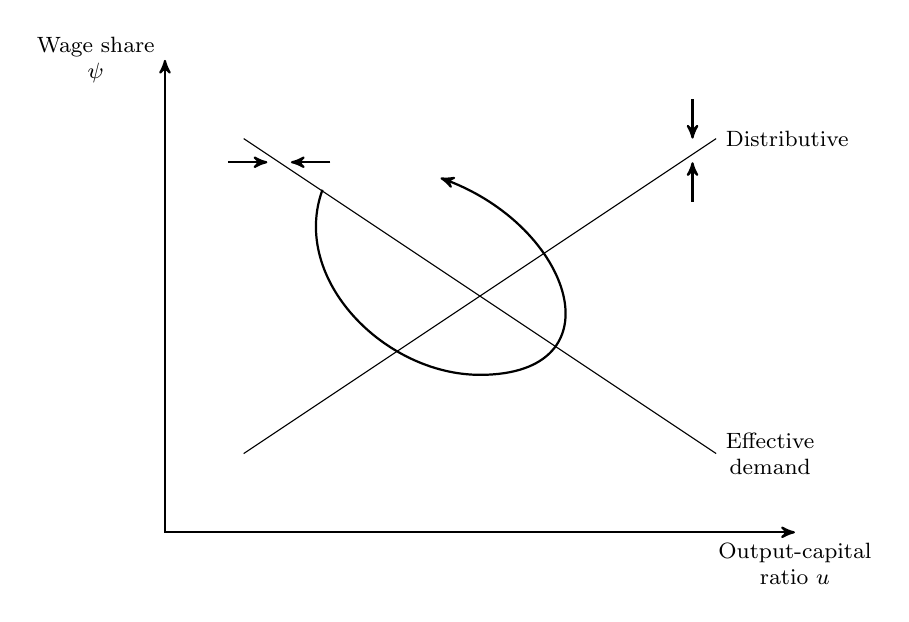
\begin{tikzpicture}

        % Axes
        \draw [<->,thick] (0,6) node[axes, align=center] (yaxis) [left] {Wage share\\$\psi$} |- (8,0) node[axes, align=center] (xaxis) [below] {Output-capital\\ratio $u$};

        % Demand and distributive curves
        \draw (1,1) -- (7,5) node [ddcross] (dist) [right] {Distributive};
        \draw (1,5) -- (7,1) node [ddcross, align=center] (demand) [right] {Effective\\demand};

        % Path
        \draw [->,thick] (2,4.35) to[out=250, in=180] (4,2) to[out=0, in=340, looseness=1.8] (3.5,4.5);

        % Arrows
        \draw [->, thick] (0.8, 4.7) -- (1.3, 4.7);
        \draw [->, thick] (2.1, 4.7) -- (1.6, 4.7);
        \draw [->, thick] (6.7, 4.2) -- (6.7, 4.7);
        \draw [->, thick] (6.7, 5.5) -- (6.7, 5);


\end{tikzpicture}
\end{document}
